\section{Análise de Resultados}

De forma a analisar os resultados obtidos experimentalmente começou-se por representar graficamente as medições da diferenca de potencial em função do tempo.

Na \cref{gra:carga} encontram-se representados os dados da \cref{tab:carga}, correspondentes ao carregamento do condensador.
\begin{figure}[!ht]
	\centering
	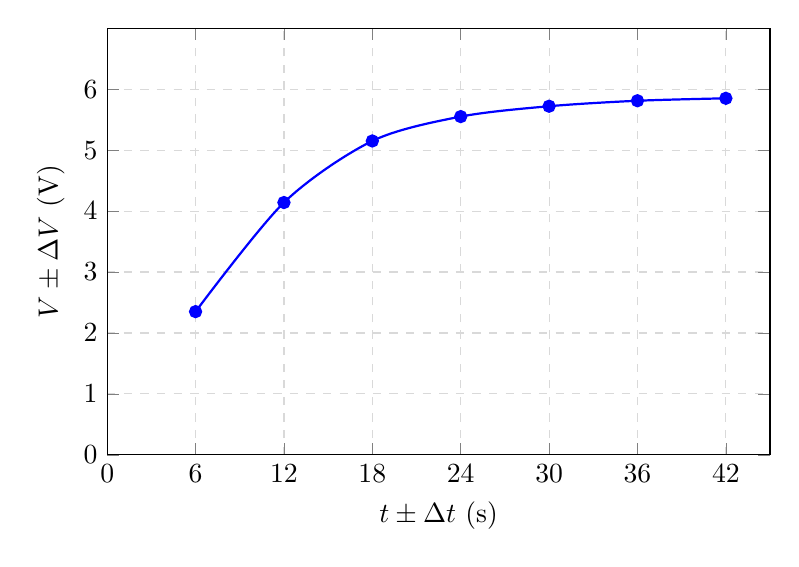
\begin{tikzpicture}
		\begin{axis}[
				% title={Capacitor Charging Curve},
				xlabel={$t \pm \Delta t$ (\unit{s})},
				xmin=0, xmax=45,
				ymin=0, ymax=7,
				xtick={0, 6, 12, 18, 24, 30, 36, 42},
				ytick={0, 1, 2, 3, 4, 5, 6},
				grid=major,
				grid style={dashed, gray!30},
				width=10cm,
				height=7cm,
				legend pos=south east,
				ylabel={$V \pm \Delta V$ (\unit{V})},
				/pgf/number format/read comma as period % Handles the comma in your data
			]

			% Plotting the data points from your table
			\addplot[
				color=blue,
				mark=*,
				smooth, % Draws a smooth curve between points
				thick
			]
			coordinates {
					(6, 2.35)
					(12, 4.14)
					(18, 5.15)
					(24, 5.55)
					(30, 5.72)
					(36, 5.81)
					(42, 5.85)
				};

			% \addlegendentry{Experimental Data}

		\end{axis}
	\end{tikzpicture}
	\caption{Voltagem em função do tempo - Carga}
	\label{gra:carga}
\end{figure}


Na \cref{gra:descarga} apresentam-se os dados de voltagem ao longo do tempo vindos da \cref{tab:descarga}, durante a descarga do condensador.
\begin{figure}[!ht]
	\centering
	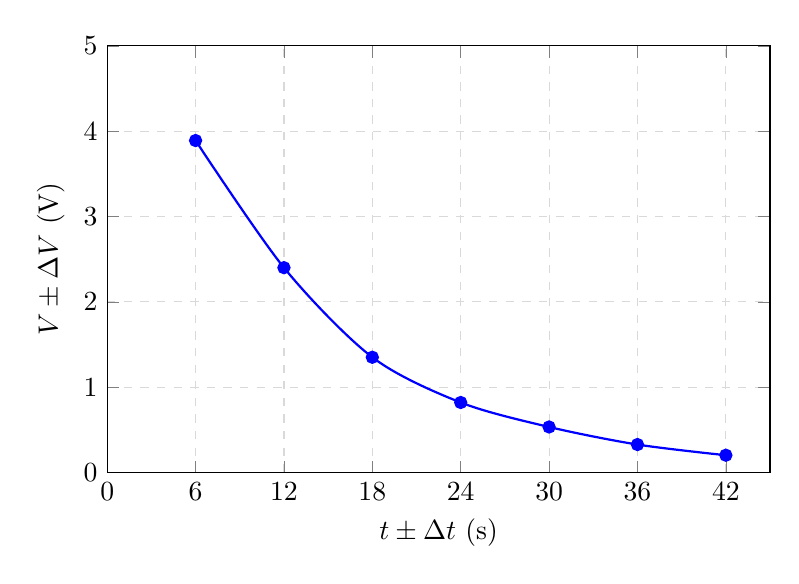
\begin{tikzpicture}
		\begin{axis}[
				% title={Capacitor Charging Curve},
				xlabel={$t \pm \Delta t$ (\unit{s})},
				ylabel={$V \pm \Delta V$ (\unit{V})},
				xmin=0, xmax=45,
				ymin=0, ymax=5,
				xtick={0, 6, 12, 18, 24, 30, 36, 42},
				ytick={0, 1, 2, 3, 4, 5, 6},
				grid=major,
				grid style={dashed, gray!30},
				width=10cm,
				height=7cm,
				legend pos=south east,
				/pgf/number format/read comma as period % Handles the comma in your data
			]

			% Plotting the data points from your table
			\addplot[
				color=blue,
				mark=*,
				smooth, % Draws a smooth curve between points
				thick
			]
			coordinates {
					(6, 3.89)
					(12, 2.40)
					(18, 1.35)
					(24, 0.820)
					(30, 0.533)
					(36, 0.327)
					(42, 0.202)
				};

			% \addlegendentry{Experimental Data}

		\end{axis}
	\end{tikzpicture}
	\caption{Voltagem em função do tempo - Descarga}
	\label{gra:descarga}
\end{figure}


Em ambos os casos obseva-se uma tendência exponencial, de acordo com as previsões teoricas das \crefrange{place}{holder}



\subsection{Linearização para o processo de carga}

A tensão nos terminais do condensador durante o processo de carga é dada pela equação (1):

\begin{equation}
V(t) = \varepsilon\, (1 - e^{-t/\tau_c})   
\end{equation}

Onde $\varepsilon$ é a tensão da fonte e $\tau_c$ é constante do tempo de carga.

\begin{align*}
&\frac{V(t)}{\varepsilon} = 1 - e^{-t/\tau_c} \\
&\Leftrightarrow 1 - \frac{V(t)}{\varepsilon} = e^{-t/\tau_c}\\
&\Leftrightarrow \ln\left(1 - \frac{V(t)}{\varepsilon}\right) = - \frac{t}{\tau_c}\\
\end{align*}

Chega-se então à relação de proporcionalidade direta, da forma $y = mx$, onde $y = \ln\left(1 - \frac{V(t)}{\varepsilon}\right)$, $x = t$ e $m = -\frac{t}{\tau_c}$


\subsection{Linearização para o processo de descarga}

Já no processo de descarga, a expressão para a tensão nos terminais do condensador em função do tempo é dada pela equação (2):

\begin{equation}
V(t) = \varepsilon\, e^{-t/\tau_d}   
\end{equation}

De forma análoga ao processo de carga:

\begin{align*}
&\frac{V(t)}{\varepsilon} = e^{-t/\tau_d} \\
&\Leftrightarrow \quad \frac{V(t)}{\varepsilon} = e^{-t/\tau_d} \\
&\Leftrightarrow\ln\left(\frac{V(t)}{\varepsilon}\right) = - \frac{t}{\tau_d}\\
&\Leftrightarrow \quad V(t) - \varepsilon = - \frac{t}{\tau_d}\\
&\Leftrightarrow \quad V(t) = \varepsilon - \frac{t}{\tau_d}\\
\end{align*}

Chega-se então à relação de proporcionalidade direta, da forma $y = mx$, onde $y = \ln\left(\frac{V(t)}{\varepsilon}\right)$, $x = t$ e $m = -\frac{t}{\tau_d}$